%%%%%%%%%%%%%%%%%%%%%%%%%%%%%%%%%%%%%%%%%%%%%%%%%%%%%%%%%%%%%%%%%%%%%%%%%%%%%%%%%%%%%%%%%%%%%%%%%%%%%%%%%%%%%%%%%%%%%%%%%%%%%%%%%%%%%%%%%%%%%%%%%%%%%%%%%%%
% This is just an example/guide for you to refer to when submitting manuscripts to Frontiers, it is not mandatory to use Frontiers .cls files nor frontiers.tex  %
% This will only generate the Manuscript, the final article will be typeset by Frontiers after acceptance.
%                                              %
%                                                                                                                                                         %
% When submitting your files, remember to upload this *tex file, the pdf generated with it, the *bib file (if bibliography is not within the *tex) and all the figures.
%%%%%%%%%%%%%%%%%%%%%%%%%%%%%%%%%%%%%%%%%%%%%%%%%%%%%%%%%%%%%%%%%%%%%%%%%%%%%%%%%%%%%%%%%%%%%%%%%%%%%%%%%%%%%%%%%%%%%%%%%%%%%%%%%%%%%%%%%%%%%%%%%%%%%%%%%%%

%%% Version 3.4 Generated 2022/06/14 %%%
%%% You will need to have the following packages installed: datetime, fmtcount, etoolbox, fcprefix, which are normally inlcuded in WinEdt. %%%
%%% In http://www.ctan.org/ you can find the packages and how to install them, if necessary. %%%
%%%  NB logo1.jpg is required in the path in order to correctly compile front page header %%%

\documentclass[utf8]{FrontiersinHarvard} % for articles in journals using the Harvard Referencing Style (Author-Date), for Frontiers Reference Styles by Journal: https://zendesk.frontiersin.org/hc/en-us/articles/360017860337-Frontiers-Reference-Styles-by-Journal

\usepackage{url,hyperref,lineno,microtype,subcaption}
\usepackage[onehalfspacing]{setspace}

\linenumbers

% Leave a blank line between paragraphs instead of using \\

\def\keyFont{\fontsize{8}{11}\helveticabold }
\def\firstAuthorLast{Lee {et~al.}} %use et al only if is more than 1 author
\def\Authors{Jover Lee\,$^{1,\dagger}$, James Hadfield\,$^{1,\dagger}$, Allison Black\,$^{2}$, Thomas R. Sibley\,$^{1}$, Richard A. Neher\,$^{3,4}$, Trevor Bedford\,$^{1,5}$, and John Huddleston\,$^{1,*}$}
% Affiliations should be keyed to the author's name with superscript numbers and be listed as follows: Laboratory, Institute, Department, Organization, City, State abbreviation (USA, Canada, Australia), and Country (without detailed address information such as city zip codes or street names).
% If one of the authors has a change of address, list the new address below the correspondence details using a superscript symbol and use the same symbol to indicate the author in the author list.
\def\Address{$^{1}$Vaccine and Infectious Disease Division, Fred Hutchinson Cancer Center, Seattle, WA, USA \\
  $^{2}$Chan Zuckerberg Initiative, CA, San Francisco, CA, USA \\
  $^{3}$Biozentrum, Universität Basel, Switzerland \\
  $^{4}$Swiss Institute of Bioinformatics, Switzerland \\
  $^{5}$Howard Hughes Medical Institute, Seattle, WA, USA \\
  $^{\dagger}$These authors contributed equally to this work and share first authorship}
% The Corresponding Author should be marked with an asterisk
% Provide the exact contact address (this time including street name and city zip code) and email of the corresponding author
\def\corrAuthor{John Huddleston}
\def\corrEmail{jhuddles@fredhutch.org}

\begin{document}
\onecolumn
\firstpage{1}

\title[Joint visualization of flu data]{Joint visualization of seasonal influenza serology and phylogeny to inform vaccine strain selection}

\author[\firstAuthorLast ]{\Authors} %This field will be automatically populated
\address{} %This field will be automatically populated
\correspondance{} %This field will be automatically populated

\extraAuth{}% If there are more than 1 corresponding author, comment this line and uncomment the next one.
%\extraAuth{corresponding Author2 \\ Laboratory X2, Institute X2, Department X2, Organization X2, Street X2, City X2 , State XX2 (only USA, Canada and Australia), Zip Code2, X2 Country X2, email2@uni2.edu}

\maketitle

\begin{abstract}

\section{}

Seasonal influenza vaccines must be updated regularly to account for mutations that allow influenza viruses to escape our existing immunity.
A successful vaccine should represent the genetic diversity of recently circulating viruses and induce antibodies that effectively prevent infection by those recent viruses.
Thus, linking the genetic composition of circulating viruses and the serological experimental results measuring antibody efficacy is crucial to the vaccine design decision.
Historically, genetic and serological data have been presented separately in the form of static visualizations of phylogenetic trees and tabular serological results to identify vaccine candidates.
To simplify this decision-making process, we have created an interactive tool for visualizing serological data that has been integrated into Nextstrain’s real-time phylogenetic visualization framework, Auspice.
We show how the combined interactive visualizations may be used by decision-makers to explore the relationships between complex data sets for both prospective vaccine strain selection and retrospectively exploring the performance of vaccine strains.

\tiny
 \keyFont{ \section{Keywords:} keyword, keyword, keyword, keyword, keyword, keyword, keyword, keyword} %All article types: you may provide up to 8 keywords; at least 5 are mandatory.
\end{abstract}

\section{Introduction}

Seasonal influenza A/H3N2 viruses primarily evolve by acquiring mutations that allow them to escape antibodies from previous infections or vaccinations \citep{Petrova2018}.
This process, known as antigenic drift, changes the appearance of viral surface proteins hemagglutinin and neuraminidase.
Hemagglutinin (HA) is the primary target of our adaptive immunity and the primary component of the seasonal influenza vaccine.
Therefore, continued antigenic drift in HA necessitates regular updates to the seasonal influenza vaccine.
The World Health Organization (WHO) Global Influenza Surveillance and Response System (GISRS) collects HA genome sequences and performs experimental measurements to track antigenic drift throughout the year \citep{Morris:2017ea}.
HA genome sequences reveal ``clades'' or groups of recent influenza viruses that descend from a common ancestor and share the same mutations that may contribute to antigenic drift.
Experimental measurements of antigenic drift quantify how well viruses from different clades can escape detection by antibodies against vaccine candidates.

The gold standard of these experimental measurements is the hemagglutination inhibition (HI) assay \citep{hirst1943studies}.
HI assays measure the minimum concentration or ``titer'' of antibodies required to prevent a given test virus from binding to red blood cells.
Typically, antibodies come from previously uninfected ferrets who are then infected with a specific reference virus (e.g., a vaccine candidate).
Each HI assay requires a series of two-fold dilutions of ferret antibodies to determine the minimum titer that inhibits binding.
The higher the antibody titer required to prevent binding, the more antigenically drifted the test virus is from the reference virus.
To enable comparison between measurements from different reference viruses, researchers normalize titers by the titer required to inhibit the reference virus itself and convert values to a $\log_{2}$ scale \citep{Neher:2016hy}.
The resulting values represent the magnitude of antigenic distance between a given reference virus and other test viruses.
Traditionally, viruses with an antigenic distance greater than $2\log_{2}$ units are considered antigenically distinct \citep{Katz2011}.

To understand long-term patterns of antigenic drift, researchers have summarized these pairwise antigenic distances with statistical or visual representations.
For example, antigenic cartography places high-dimensional antigenic distances in a two-dimensional space using multidimensional scaling \citep{Smith:2004jc,Bedford:2014bf}.
These map-like visualizations reveal long-term trends in antigenic drift within seasonal influenza lineages like the punctuated emergence of new antigenic clusters every few years.
However, antigenic cartography is less suited to representations of short-term antigenic drift on the same time scale as annual vaccine updates in each hemisphere.

To understand short-term patterns of antigenic drift that would require an update to the vaccine, WHO decision makers need to answer specific questions.
These include a) which available vaccine candidates require additional titer measurements against currently circulating clades, b) which vaccine candidates have the lowest antigenic distance to each clade, and c) what is the antigenic diversity of recent clades.
In practice, decision makers must choose the next vaccine candidate from a small pool of viable options.
The best candidate will have titer measurements against all current clades and have the lowest antigenic distance across these clades.
Such candidates are said to effectively ``cover'' currently circulating clades.
Determining the vaccine candidate that most effectively covers recent clades requires a direct comparison of antigenic distances across all available vaccine candidates.

We have previously developed two alternate visualizations of antigenic data to answer these questions and inform vaccine selection through reports to the WHO \citep{BedfordWHO2018,BedfordWHO2019}.
The first visualization is an interactive phylogenetic view implemented in the genomic epidemiology tool \emph{nextflu} \citep{NeherBedford2015,NeherBedford2018}.
When the user selects a given reference virus from the phylogeny (by selecting a ``gear'' icon), the tool plots the pairwise antigenic distances between that reference and the corresponding test viruses in the tree using color to represent the distance values (Figure~\ref{fig:1}A).
This representation reveals clades that the selected reference virus may or may not cover and which clades lack measurements against the reference.
While this view provides phylogenetic context of titer measurements and shows the individual pairwise measurements, it does not support direct comparison of antigenic distances from different vaccine candidates.
Instead, users must quickly toggle between different vaccine candidates in the tree to get a sense of how well different viruses may perform.

To complement the interactive phylogenetic visualization, we also developed a static heatmap visualization that summarizes the mean antigenic distances between a subset of vaccine candidates and all tests viruses within each extant clade.
The resulting heatmaps use the x-axis to encode the names of major clades, the y-axis to encode the names of reference viruses, and color and text to encode the mean $\log_{2}$ distance between a given reference virus and corresponding test viruses in each clade (Figure~\ref{fig:1}B).
These heatmaps allow decision makers to directly compare average antigenic distances for different vaccine candidates and quantify how these candidates cover extant clades.
However, these heatmaps suffer reduced expressiveness by encoding the most valuable quantitative data with color instead of a spatial scale.
Additionally, this view shows a summary statistic instead of the underlying distributions of the data, concealing the number and variance of measurements for each reference virus.

\section{Methods}

\subsection{Visual design}

To overcome the limitations of existing antigenic visualizations, we applied user-driven design based on the goals of decision makers described above and used standard visual design principles to produce a more expressive and effective visualization for influenza virologists.
Of the two previous visualizations we developed, the static heatmaps addressed the most user goals except for communicating which extant clades were missing measurements.
Both previous visualizations effectively obscure or hide the underlying distributions of the raw data.
Since visualization of these distributions can improve confidence during the decision making process, we treated the need to view these distributions as an auxillary user goal \citep{}.

In the context of visual design principles, both the phylogenetic and heatmap views encode the most relevant quantitative data of antigenic distance with color.
However, quantitative data can be more effectively represented by positional encodings (e.g., x- or y-axis positions) whereas nominal data (e.g., phylogenetic clades) can be effectively encoded with color \citep{Mackinlay1986}.
In the phylogenetic view, the two available positional axes represent time and the unitless phylogenetic position of nodes, neither of which are relevant to the user goals described above.
In the heatmaps, the two positional axes encode two nominal data types.

We reasoned that we could make a more effective visualization that addressed all user goals by simply changing the encoding of data in the heatmaps.
To this end, we swapped the encoding of antigenic distances and test clades, encoding quantitative distances on the x-axis positional scale and encoding nominal test clades with a color scale.
The positional encoding of antigenic distances allowed us to visually encode relevant thresholds for decision making (i.e., $x = 2\log_{2}$), show all available measurements for each reference virus at once, and display a summary statistic (mean and standard deviation of antigenic distances) for each reference virus.
We retained the encoding of nominal reference virus names on the y-axis, since most user goals require comparison of distances between specific vaccine candidates.

\subsection{Data curation}

\subsection{Implementation}

We implemented this design as a new interactive measurements panel within Nextstrain's visualization tool, Auspice, which is freely available on Github (\url{https://github.com/nextstrain/auspice}) under the AGPLv3 license.
The visualization requires a minimum of two JavaScript Object Notation (JSON) files that are produced by the Nextstrain bioinformatics toolkit, Augur \citep{Huddleston2021}.
The phylogeny tree is provided via a dataset JSON file produced by \texttt{augur export v2} and the measurements data is provided via a measurements sidecar JSON file produced by \texttt{augur measurements}.
The measurements file must follow a specific filename format for Auspice to link it to the dataset file, where the dataset filename is \texttt{\$\{name\}.json} and the measurements filename must be \texttt{\$\{name\}\_measurements.json}.
The application can be cloned and run locally or users can use Auspice through two public websites.
Users can drag and drop dataset and measurements files onto \url{https://auspice.us/} to visualize the data in their own browser.
If users want to share their visualizations publicly, they can make their files available through a public GitHub repository and view the visualizations through \url{https://nextstrain.org/community/}.
The visualization for this paper has been shared via Nextstrain community and can be viewed at \url{https://nextstrain.org/community/blab/measurements-panel/flu/seasonal/h3n2/ha}.

\section{Results}

\subsection{Interactive visualization of titer measurements}

Our goal for incorporating the measurements panel into Auspice is to allow users to explore relationships between the genetic and serology data in one interactive visualization.
Test viruses of the titer data are directly linked to the viruses displayed in the phylogeny tree via their strain names to ensure that any interactions with the tree are also applied to the titer data.
Filters applied to the tree via the date slider (Figure~\ref{fig:2}a), the data filter (Figure~\ref{fig:2}d), or directly filtering the tree by clicking on branches and tips also filters the titer data.
This allows users to easily focus on a subset of the titer measurements that is phylogenetically relevant, such as examining the measurements of viruses in recently circulating clades.
The measurements are colored by the same coloring attribute (Figure~\ref{fig:2}b) as the phylogeny tree, adding the legend values (Figure~\ref{fig:2}c) as another dimension of data to the titer measurements.
This is especially useful for applying genotypes to the titer data, allowing users to reveal potential cause and effect relationships between mutations and titer measurements.

The measurements JSON can include multiple collections of titers for a single phylogeny tree and users can use the collection dropdown (Figure~\ref{fig:2}e) to change the collection displayed.
This allows users to examine different sets of data for the same phylogeny tree such as changing between cell and egg passaged virus titers.
Users can change the subplots displayed by specify different grouping categories for the measurements using the group by dropdown (Figure~\ref{fig:2}f).
In our case, the most useful grouping is the reference strain so that we can compare the reference strain (Figure~\ref{fig:2}j) to the displayed measurements.
The data display can be toggled between mean with standard deviation and the raw individual measurements (Figure~\ref{fig:2}g).
When viewing the mean with standard deviation, the measurements are grouped by their coloring values to calculate the mean for each coloring value.
The overall mean for each grouping can be toggled (Figure~\ref{fig:2}h) to show the overall mean with standard deviation that is not split into the coloring groups.
The measurements threshold can be toggled (Figure~\ref{fig:2}i) for a clear demarcation of a threshold value.
For titer measurements, this is the $\log_{2}$ distance of 2 to easily show when titer measurements are considered antigenically distinct (Figure~\ref{fig:2}k).

\subsection{Case study 1: Retrospective vaccine strain selection in Fall 2009}

The vaccine selection decisions for the 2010-11 northern hemisphere influenza season ocurred in the fall of 2009.
A phylogenetic tree using publicly available data from \citep{Bedford:2014bf} (Figure~\ref{fig:3}A) identifies three potentially co-circulating clades 173Q, 144K and 158N/189K, with 173Q dominant in the previous season and 144k dominant in the 2009 southern hemisphere season.
The H3N2 vaccine used a A/Brisbane/10/2007-like virus for each of those two seasons, part of the earlier 140I clade which not seen in large numbers since the 2007/8 season.
Comparing the current vaccine choice to a both an older reference sera (A/Wisconsin/67/2005) and a newer sera (A/Perth/16/2009) indicates a large variability in the normalized HI scores against test viruses from different clades available by the selection deadline (Figure~\ref{fig:3}B) (Todo explain the choice of these reference sera).
These data indicate that both A/Wisconsin/67/2005 and A/Brisbane/10/2007 sera have poor responses (higher normalized log2 titer values) to clades 144K and 158N/189K, whereas A/Perth/16/2009 showed more potent neutralizing ability.
Given the dominance of clade 144K in the 2009 southern hemisphere season the choice was made to recommend switching to a A/Perth/16/2009-like virus for the (H3N2) vaccine (TODO - check wording here).


Adding in data from after the vaccine selection deadline (Figure~\ref{fig:3}A,C) indicates that clade 158/189 predominated for the following H3N2 seasons in both hemispheres, and that A/Perth/16/2009 continued to provide consistently better coverage (todo: better wording?) against these strains compared with the previous vaccine choice.


A/Perth/16/2009 remained the WHO's recommended H3N2 vaccine strain for the 2010-12 southern hemisphere seasons and the 2010-11 and 2011-12 northern hemisphere seasons. Note that the actual selection process used a richer dataset which is not publicly available to include here, and as such these data should be seen as representative of the process only.


\subsection{Case study 2: Identification of genotype-specific patterns through visualization of raw data}

All else being equal, genetically similar strains will have low (better) HI titer measurements than antigenically diverged strains.
While clade definitions attempt to capture antigenic similarity, mutations may still be present within a clade which result in differing responses of reference sera to the test strains in the clade.


Clade 144V circulated between 1984 and 1992 (Figure~\ref{fig:4}A) and multiple reference sera from this clade have been used in HI assays.
Looking at two such reference sera, there is a wide distribution of titer measurements when tested against viruses from the same clade; the two sera shown in Figure~\ref{fig:4}B have titer values which range from antigenically similar to distinct.
Looking at the raw measurements themselves Figure~\ref{fig:4}C indicates a potentially bimodal distribution for the A/Shanghai/11/1987 sera, which is hidden by looking at the distribution summaries themselves.
Nextstrain allows us to interrogate the mutations observed within a clade such as 144V via a number of approaches, and the entropy panel indicates that codon HA1:135 has the highest entropy among 144V genomes, indicating that multiple amino acids are present in a large fraction of viruses here.
Coloring the data by genotype HA1:135 (Figure~\ref{fig:4}D) not only indicates that these residue changes may explain the bimodal distribution though to exist in A/Shanghai/11/1987 responses, but also indicates that this bimodality may also be present in A/Beijing/252/1989 results; these sera contain HA1:135G and HA1:135E, respectively, which is a plausible explanation for why the former has lower titer scores against HA1:135G test viruses and the later has lower titer scores against HA1:135E.
HA:135 is located in the receptor binding domain (citation needed) and is thus a very plausible driver of such distinct inhibition responses.


\section{Discussion}

\section*{Conflict of Interest Statement}
%All financial, commercial or other relationships that might be perceived by the academic community as representing a potential conflict of interest must be disclosed. If no such relationship exists, authors will be asked to confirm the following statement:

The authors declare that the research was conducted in the absence of any commercial or financial relationships that could be construed as a potential conflict of interest.

\section*{Author Contributions}

JL, TRS, TB, and JHa designed and implemented measurements panel in Auspice.
JHu and AB designed and implemented initial prototypes of interactive measurements visualizations.
JHu, AB, and RAN designed and implemented static visualizations.
JL, JHu, and JHa wrote manuscript.

\section*{Funding}
Details of all funding sources should be provided, including grant numbers if applicable. Please ensure to add all necessary funding information, as after publication this is no longer possible.

\section*{Acknowledgments}
This is a short text to acknowledge the contributions of specific colleagues, institutions, or agencies that aided the efforts of the authors.

\section*{Supplemental Data}
 \href{http://home.frontiersin.org/about/author-guidelines#SupplementaryMaterial}{Supplementary Material} should be uploaded separately on submission, if there are Supplementary Figures, please include the caption in the same file as the figure. LaTeX Supplementary Material templates can be found in the Frontiers LaTeX folder.

\section*{Data Availability Statement}
The datasets [GENERATED/ANALYZED] for this study can be found in the [NAME OF REPOSITORY] [LINK].
% Please see the availability of data guidelines for more information, at https://www.frontiersin.org/about/author-guidelines#AvailabilityofData

\bibliographystyle{Frontiers-Harvard}
\bibliography{measurements-panel}

%%% Make sure to upload the bib file along with the tex file and PDF
%%% Please see the test.bib file for some examples of references

\section*{Figure captions}

%%% Please be aware that for original research articles we only permit a combined number of 15 figures and tables, one figure with multiple subfigures will count as only one figure.
%%% Use this if adding the figures directly in the mansucript, if so, please remember to also upload the files when submitting your article
%%% There is no need for adding the file termination, as long as you indicate where the file is saved. In the examples below the files (logo1.eps and logos.eps) are in the Frontiers LaTeX folder
%%% If using *.tif files convert them to .jpg or .png
%%%  NB logo1.eps is required in the path in order to correctly compile front page header %%%

\begin{figure}[h!]
  \begin{center}
    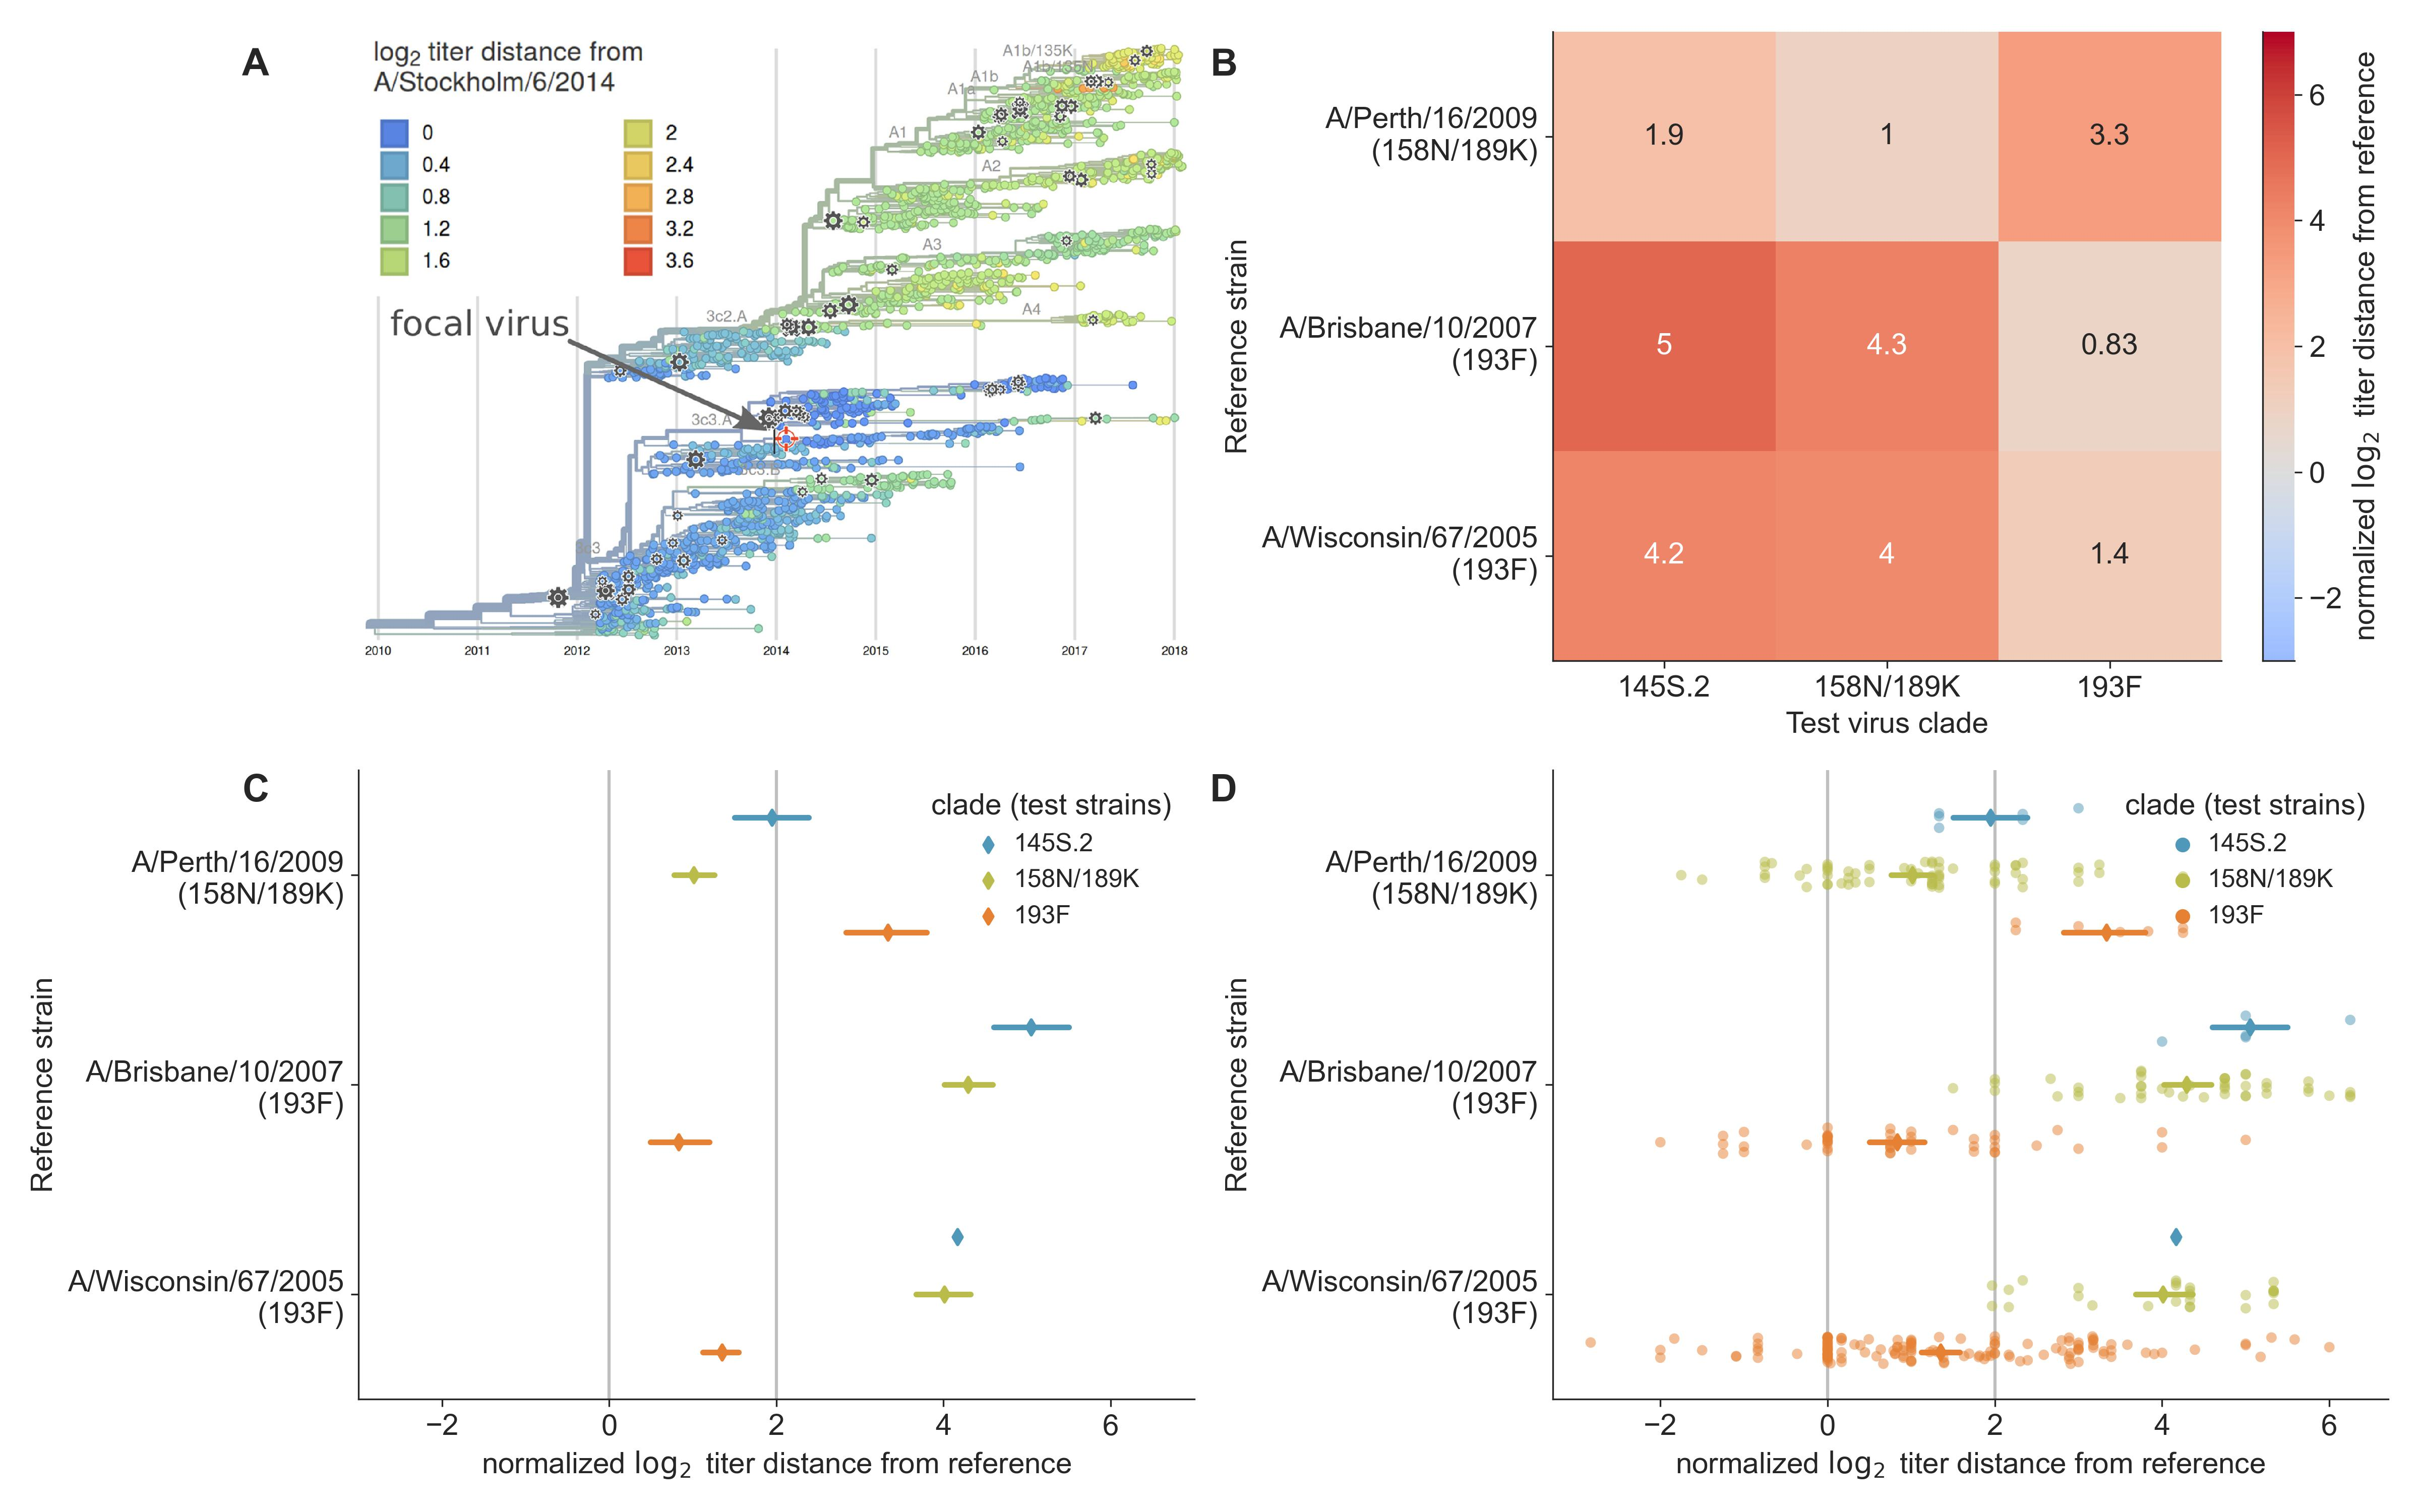
\includegraphics[width=\textwidth]{figures/figure-1-static-titer-visualizations}
  \end{center}
  \caption{
    Previous approaches to static visualization of serological data for seasonal influenza vaccine composition reports.
A) Phylogenetic visualization \citep{NeherBedford2018} allows the user to select a single vaccine candidate (e.g., A/Texas/50/2012) and see how well that strain might protect against other circulating strains in their genetic context based on the serological distance encoded by color (orange and red color indicate greater distance and less protection by the selected strain).
To compare multiple vaccine candidates, users have to select different strains manually and toggle between them.
B) Heatmap visualization of mean serological distances between multiple vaccine candidates (reference strains on the y-axis) and strains in currently circulating phylogenetic clades.
Heatmaps encode distance by color and display the distance as text, allowing the user to compare how well multiple vaccine candidates might protect against circulating strains.
C) Interval plot of mean +/- 89\% confidence interval values of serological distances between vaccine candidates (y-axis) and strains in currently circulating clades.
Unlike the heatmap visualization, the interval plot encodes serological distance with a spatial scale (the x-axis) instead of color and encodes clade membership with color instead of the spatial scale.
The vertical gray lines represent the threshold above which strains are considered antigenically distinct (x=2, solid line) and where strains are antigenically identical (x=0, dashed line).
This view allows users to compare multiple vaccine candidates, identify the candidate that protects specific clades based on a mean value to the left of the threshold at x=2, and view the variance in the underlying serological measurements.
D) Combined swarm and interval plot showing the raw pairwise measurements between each vaccine candidate and the test strains in each clade.
This view allows users to perform the same tasks as the interval plot, but it also allows users to identify how many measurements support the summary statistics for a given vaccine candidate and identify multiple modes in the raw data distribution that could indicate within-clade antigenic variation.
}\label{fig:1}
\end{figure}

\begin{figure}[h!]
  \begin{center}
    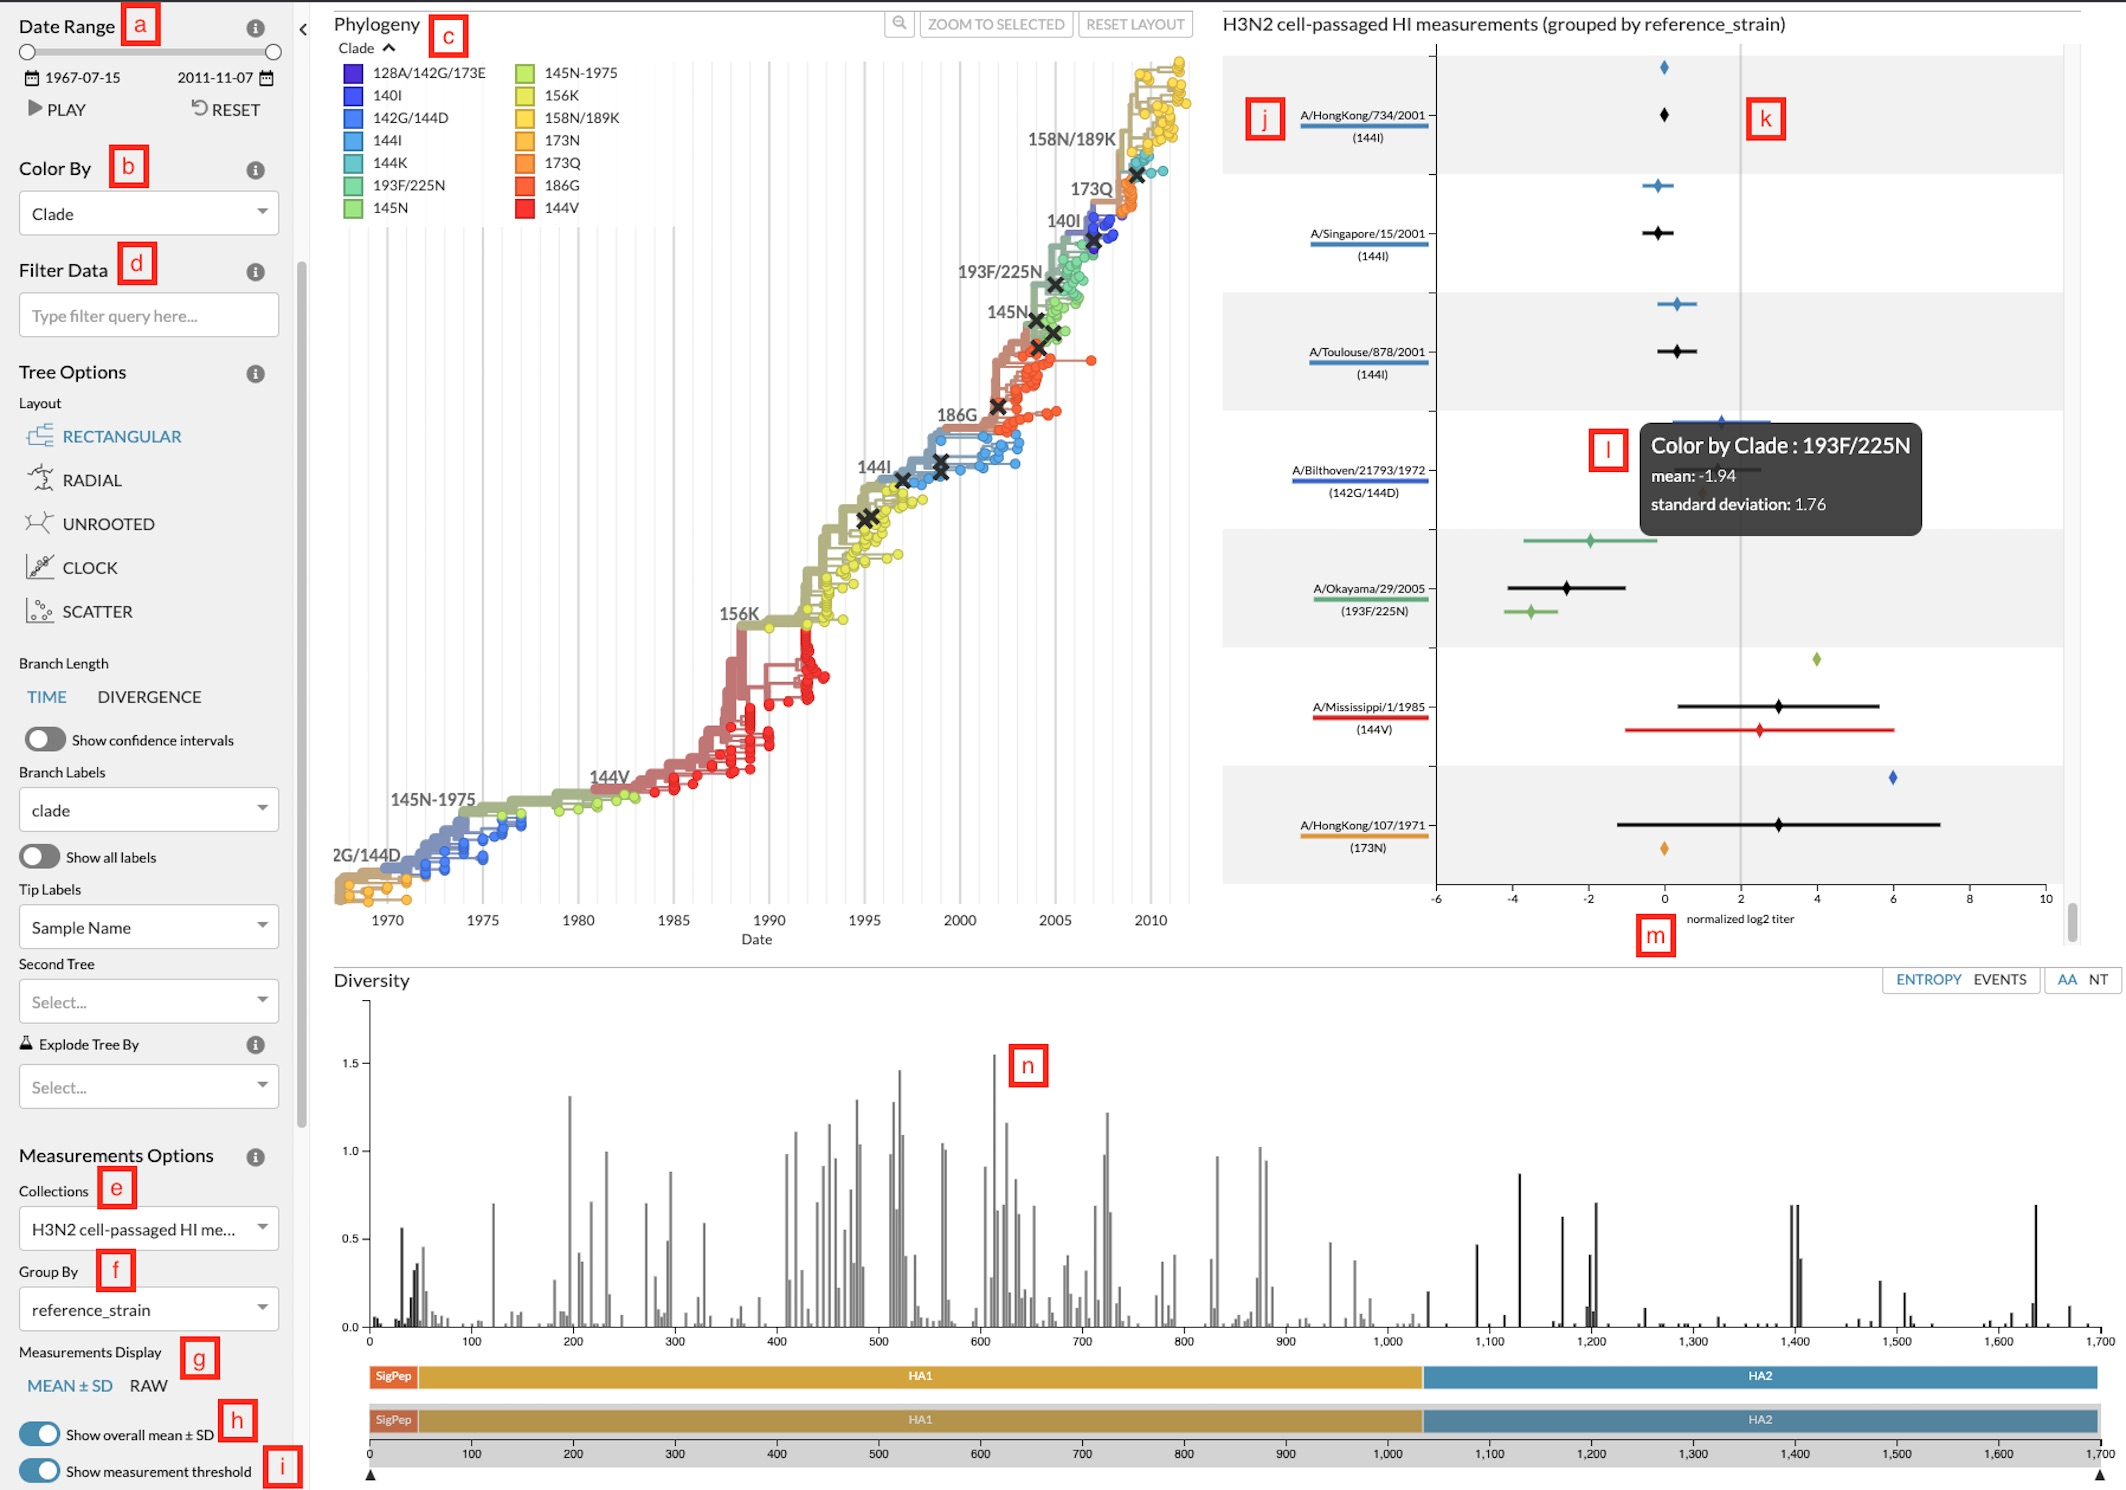
\includegraphics[width=\textwidth]{figures/figure-2-screen-shot}
  \end{center}
  \caption{
    Screenshot of Auspice with the sidebar controls, the phylogeny tree panel, and the measurements panel.
a) Date range slider to filter both tree and measurements by the test virus sample date.
b) Color-by dropdown to change the attribute to use for coloring the tree and measurements.
c) Legend for colors and their corresponding values linked to viruses in the tree and measurements.
d) Data filter search bar to filter tree and measurements data by specific attributes.
e) Measurements collection dropdown to change the collection of measurements displayed.
f) Measurements group by dropdown to change the grouping of measurements data.
g) Toggle to change measurements display between mean with standard deviation and individual raw measurements.
h) Toggle to display or hide the overall mean and standard deviation for each group.
i) Toggle to display or hide the threshold line.
j) Grouping label for each group of measurements.
This particular view uses reference viruses that are also present in the tree so the label includes the virus' corresponding color and color-by value.
k) The threshold line for titer measurements to indicate the threshold for antigenically distinct viruses.
l) The hover panel that displays more details for the hovered measurement.
This particular view hovers over a mean and standard deviation.
m) The x-axis of the measurements plot shows the range of measurements values in this collection.
  }\label{fig:2}
\end{figure}




\begin{figure}[h!]
  \begin{center}
    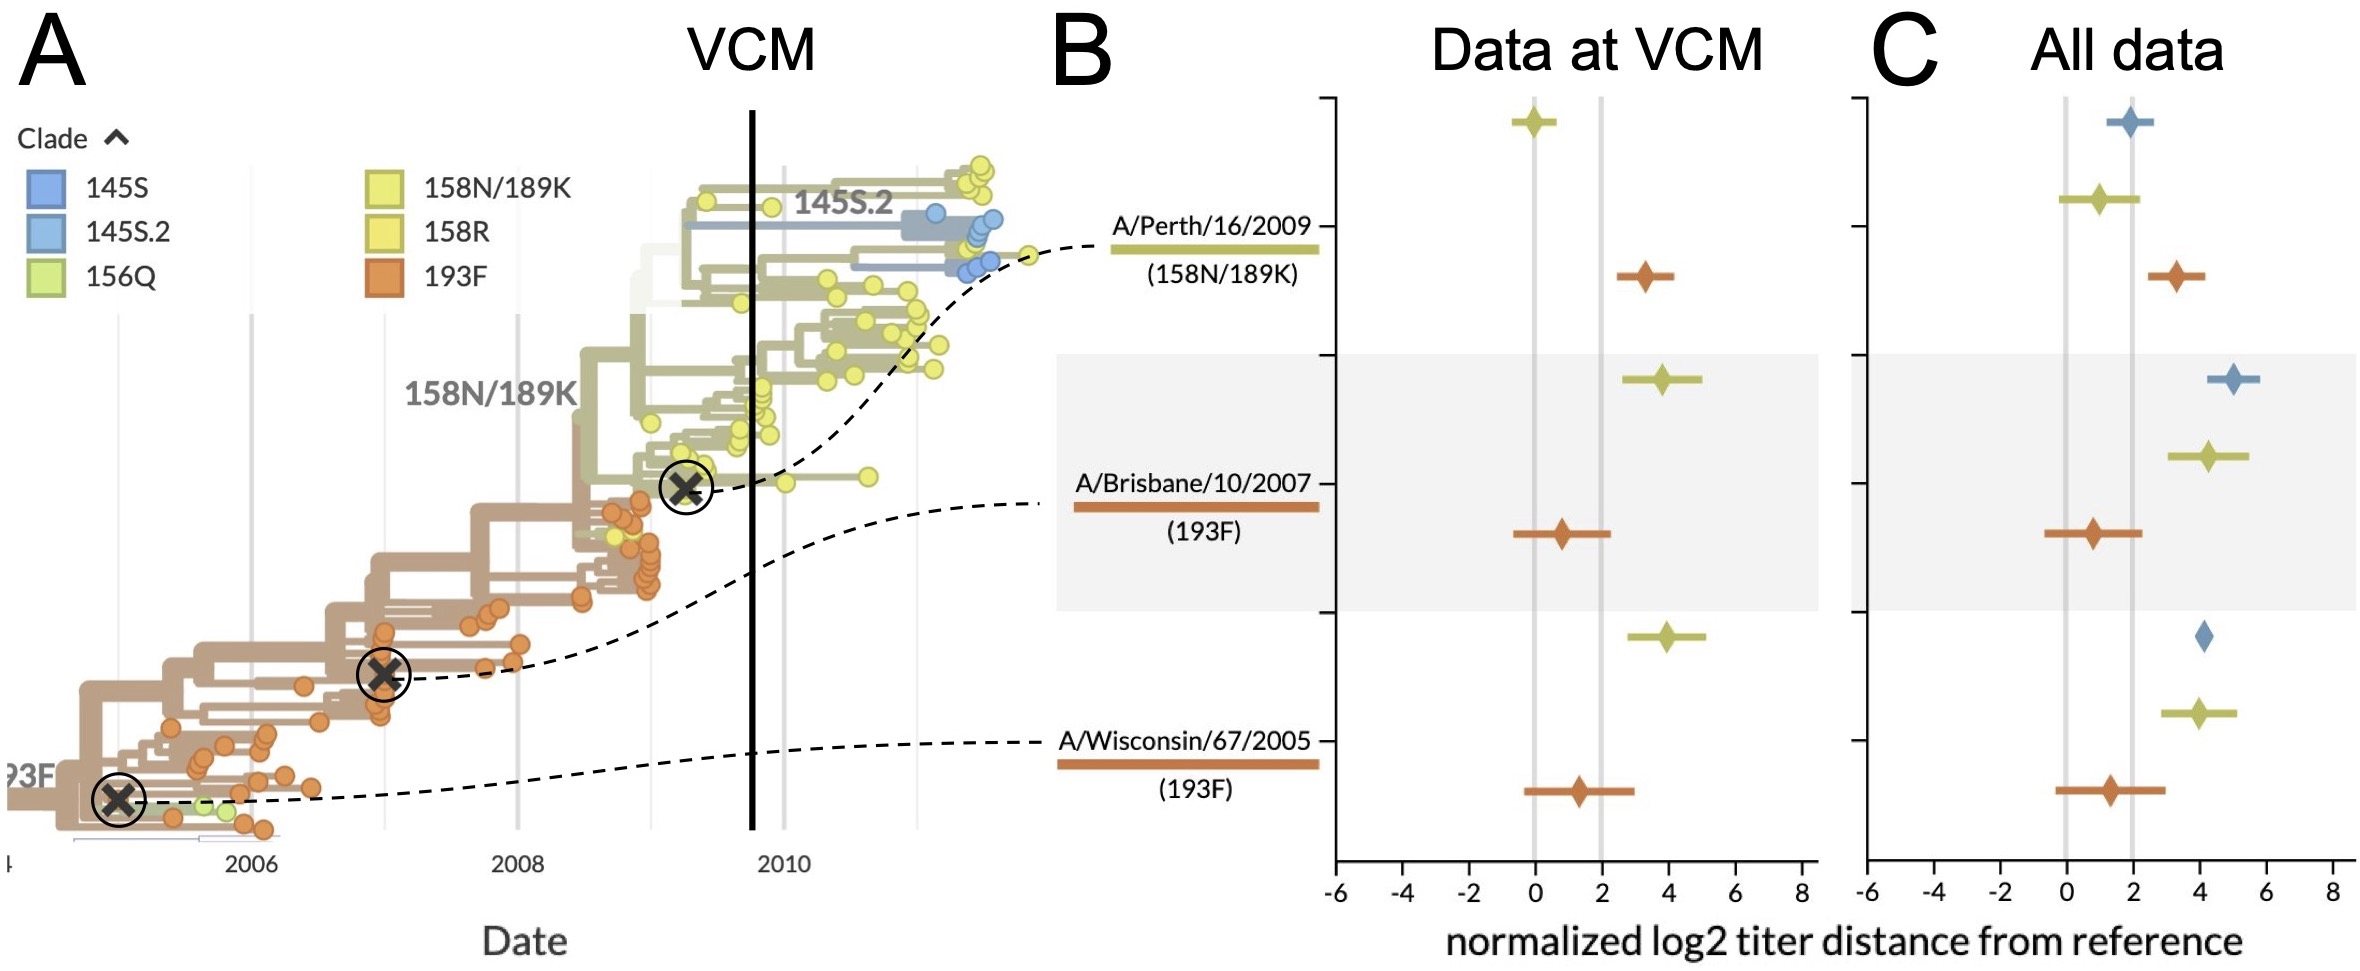
\includegraphics[width=\textwidth]{figures/figure-3.jpg}
  \end{center}
  \caption{
    Fall 2009 vaccine selection candidates.
    A) Phylogenetic tree summarizing the clade turnover. At the selection deadline clade 144K (light blue) was dominant, with A/Perth/16/2009 the candidate reference sera from this clade.
    B) Neutralization titers against three candidate vaccine strains (reference sera) using data available prior to the selection deadline.
    C) Same as (B) but including test viruses collected after the selection deadline.
    \break
    TODO change fonts, reorder reference sera etc. This can be done after the text is finalised.
    \break
    Potential todo: identify the northen hemisphere influenza seasons? Perhaps by replacing Auspice's date lines with shaded regions.
  }
  \label{fig:3}
\end{figure}



\begin{figure}[h!]
  \begin{center}
    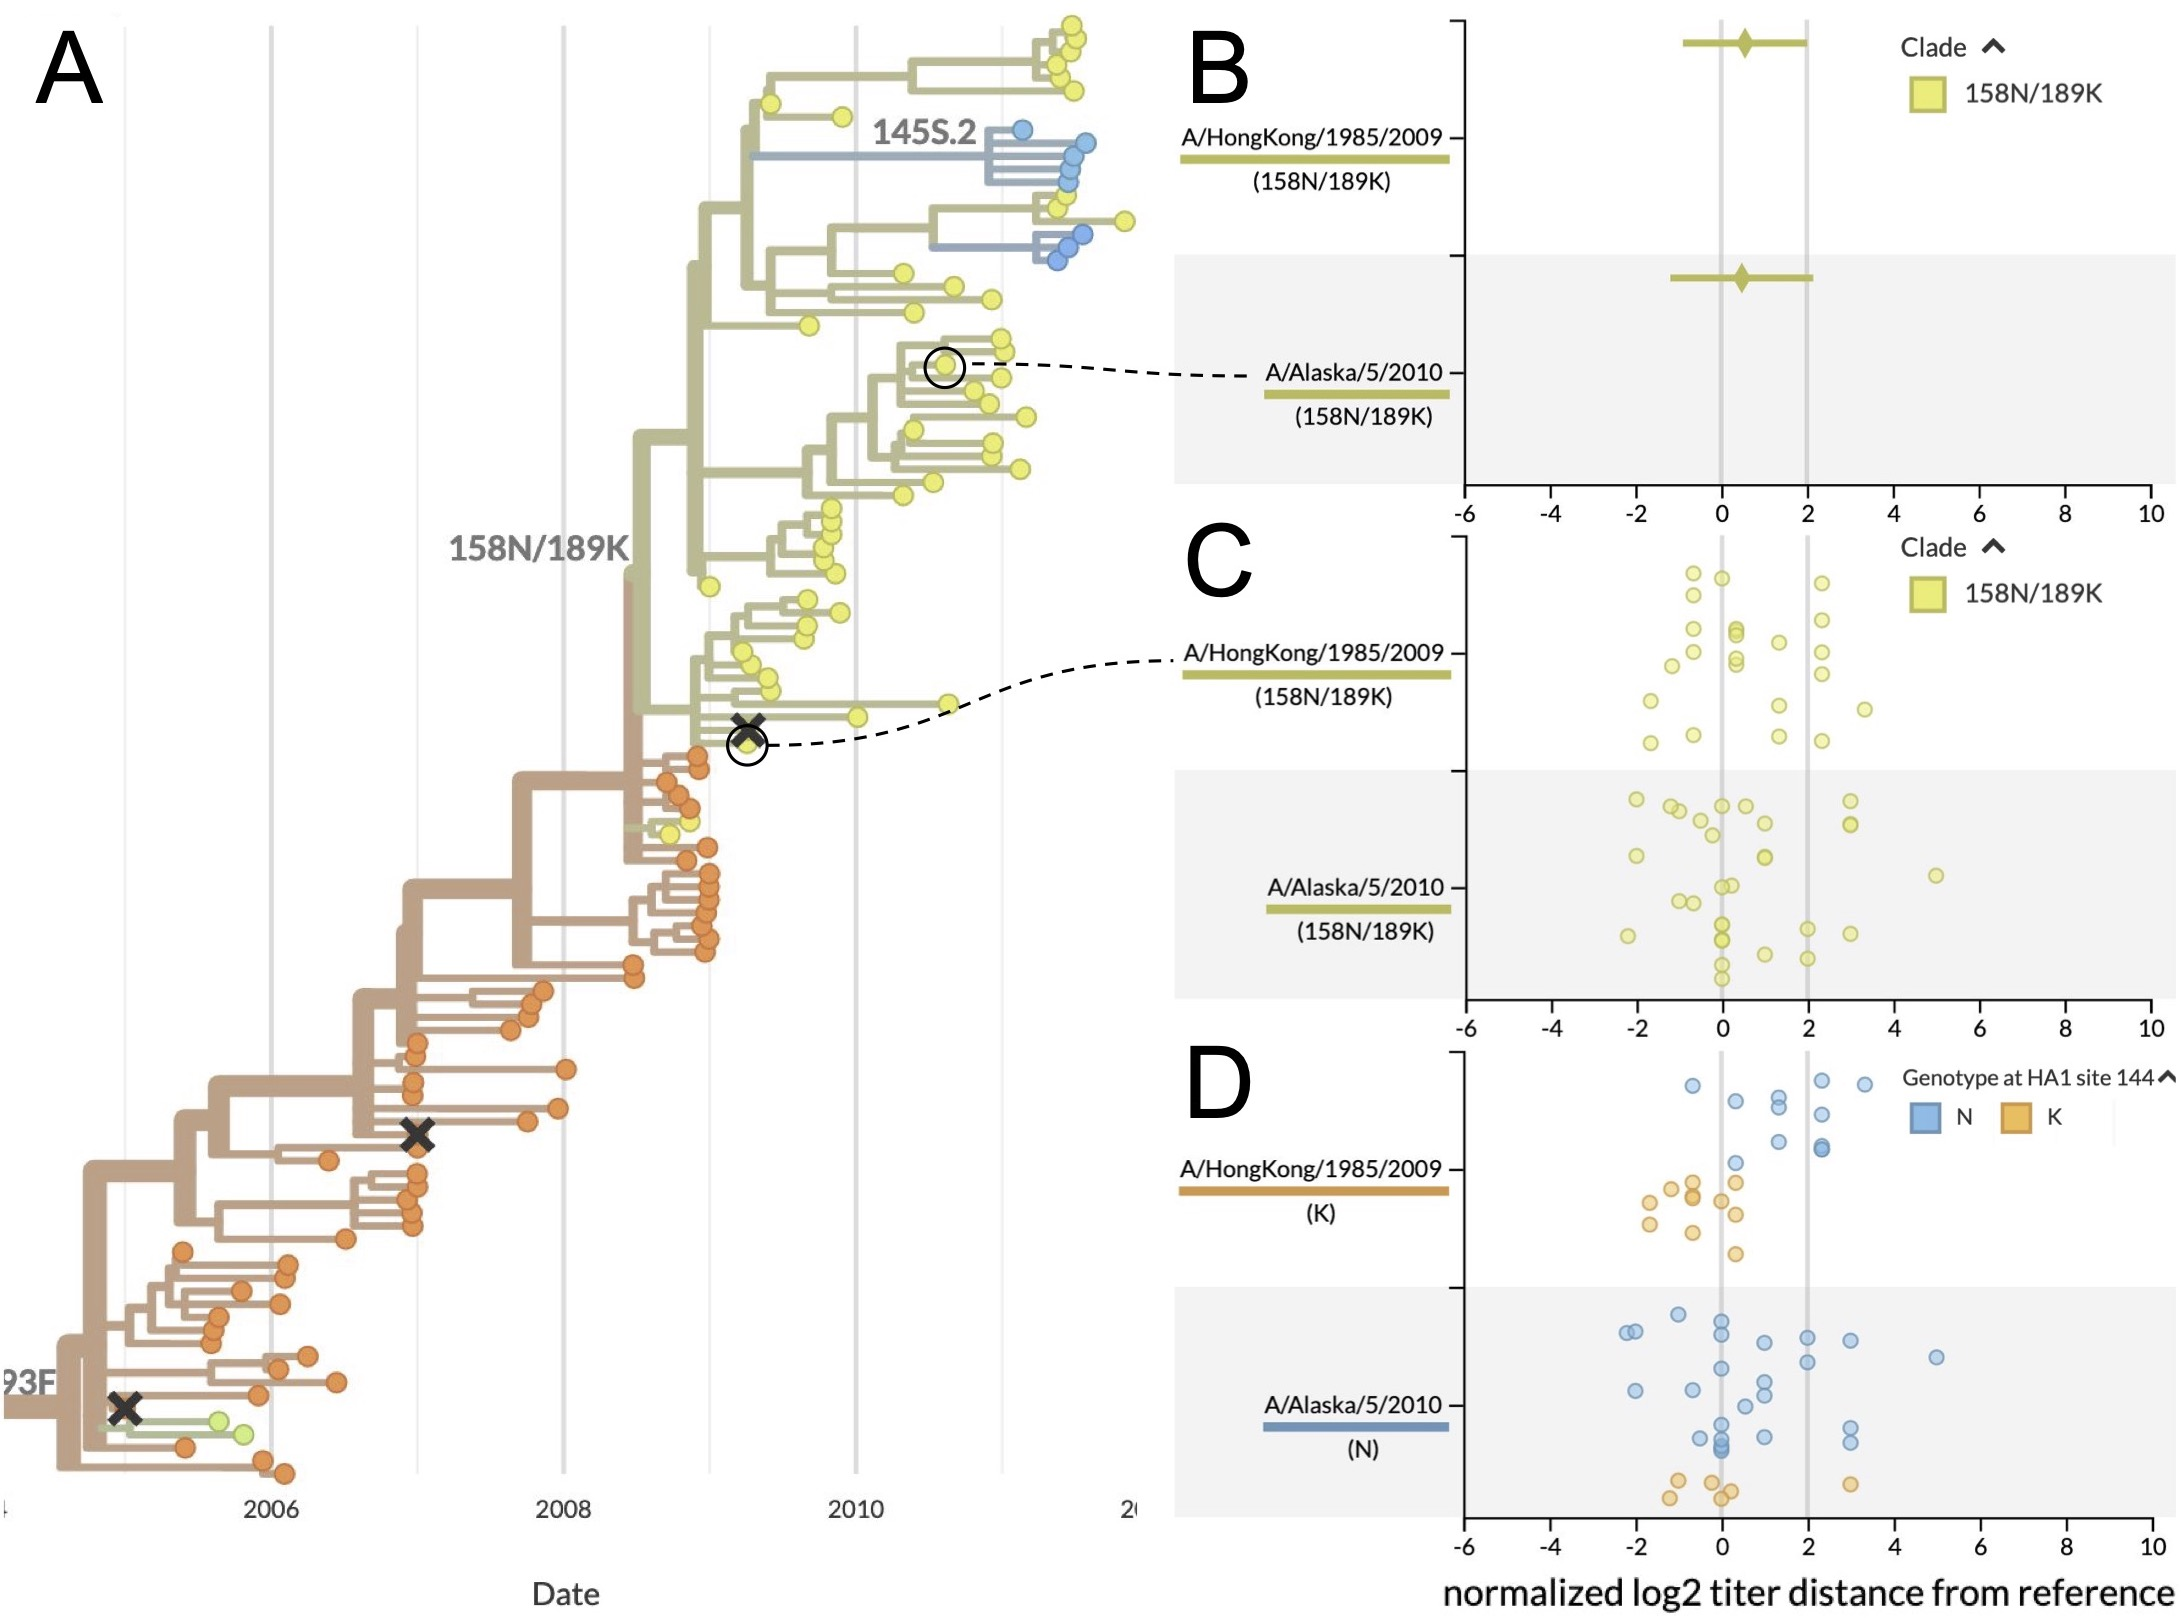
\includegraphics[width=\textwidth]{figures/figure-4.jpg}
  \end{center}
  \caption{
    Neutralization of clade 144V sera is bimodal when conditioning on RBD site 135.
    A) Summary phylogenetic tree with clade 144V highlighted.
    B) Mean titer measurements of 2 144V reference sera against 144V test viruses appear similar.
    C) Individual (raw) measurements suggest a previously hidden bimodal distribution in the measurements for the A/Shanghai/11/1987 reference strain compared to a unimodal distribution for the A/Beijing/353/1989 reference strain.
    D) When coloring by RBD site HA1:135 reveals a  potential genotype-specific explanation for the two clusters seen in the A/Shanghai/11/1987 measurements and a similar bimodal distribution in the measurements for A/Beijing/353/1989 that was not as clear when coloring raw measurements by clade alone.}
  \label{fig:4}
\end{figure}

%%% If you don't add the figures in the LaTeX files, please upload them when submitting the article.
%%% Frontiers will add the figures at the end of the provisional pdf automatically
%%% The use of LaTeX coding to draw Diagrams/Figures/Structures should be avoided. They should be external callouts including graphics.

\end{document}
